\chapter{Convolutions}
    % Authors: Rafael Moraes, Jiachen Zhu, Kabir Singh; 2019-02-19
    \section{Natural Data Properties}
    % Authors: Rafael Moraes, Jiachen Zhu, Kabir Singh; 2019-02-19
    Natural signals (e.g. audio, images, text) have 3 properties that make convolutions a good choice to process them:
    \begin{enumerate}
        \item \textbf{Stationarity}: similar patterns repeat in the data. 
        For example, in an image, similar patches appear in different locations and not all patches are equally frequent. Formally we define this as "a process or data where the mean, variance and autocorrelation structure does not change over time." More simply put, in data, we can observe stationarity when a pattern repeats over degrees of freedom.
        
        \begin{figure}[H]
        \begin{center}
        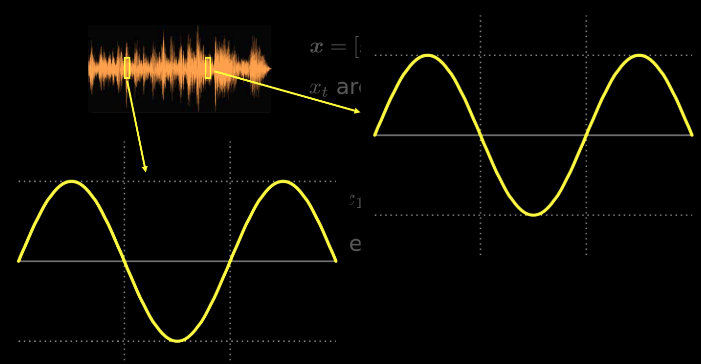
\includegraphics[width=200pt]{labs/03/images/stationarity.png}
        \end{center} 
        \captionsetup{justification=centering, margin=2cm}
        \caption{Example of stationarity - we can observe similar waveforms over different parts of one data set.}
        \end{figure}
        
        \item \textbf{Locality}:  points close to one another have more information about each other than points far apart. 
        In other words, two points far apart are less likely to have a higher correlation than two points closer to each other. 
        For example, audio signals or pixels in an image.
        
        \begin{figure}[H]
        \begin{center}
        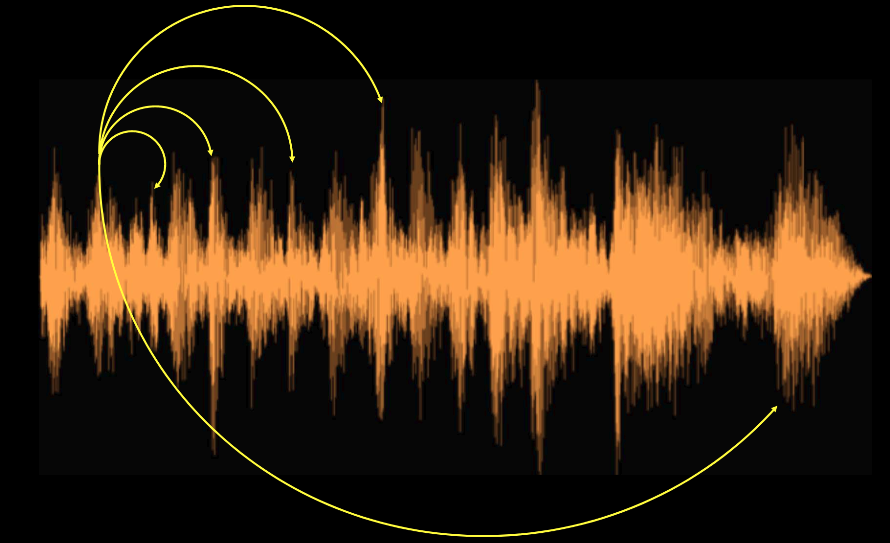
\includegraphics[width=200pt]{labs/03/images/locality.png}
        \end{center}
        \captionsetup{justification=centering, margin=2cm}
        \caption{Data points are more "relevant" to other data points nearby, less relevant as you move further away.}
        \end{figure}
        
        \item \textbf{Compositionality}: the world we live in is formed from a hierarchy of structure. Each level is composed from a group of structures from the lower levels. Complex expressions are formed by a combination of its simpler constituent expressions. For example, images are composed of pixels, pixels together form edges and color patters, these together form motifs, which then form shapes, objects, scenes and so forth.
        This implies that a good way to identify a scene, for example, is to first understand the edges and color patterns, then the motifs and so on, which translates into the convolutional layers successfully used in this task. 
        This compositionality characteristic of images was first introduced in biology, by analyzing how the human brain processes visual signals at each different stage of the visual cortex.
    \end{enumerate}
    
    \section{Exploiting The Properties}   
    % Authors: Rafael Moraes, Jiachen Zhu, Kabir Singh; 2019-02-19
    By making use of these properties, some simplifications can be introduced to our models:
    
    \begin{enumerate}
        \item \textbf{Locality \(\Rightarrow\) Sparsity}: 
    
           Since the information that is most relevant to identify a particular region of the signal (e.g. image) is close to that region, our models do not need to analyze regions far away from each region of interest. 
           Thus, in an neural network, a single unit does not need to be directly connected to a large portion of the input signal. 
            In other words, the connections can be sparse: mostly zero, except in the areas surrounding the region of interest. 
            In biology, this phenomenon is called the Receptive Field: "an individual neuron relates to a specific sensory space (e.g., the body surface, or the visual field) in which a stimulus will modify the firing of that particular neuron"; aka, neurons and their analogous 
            receptive fields are highly localized.
            
            \begin{figure}[H]
            \begin{center}
            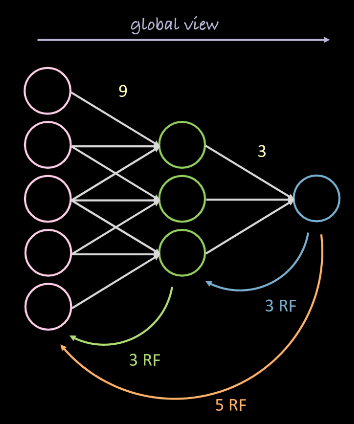
\includegraphics[width=200pt]{labs/03/images/sparsity.png}
            \end{center}
            \captionsetup{justification=centering, margin=2cm}
            \caption{Like receptive fields, we can restrict input connections from incoming layers, instead of being fully connected.}
            \end{figure}
        
        
        \item \textbf{Stationarity \(\Rightarrow\) Parameter Sharing}:
        
              Since we know only a portion of the input needs to perfuse to each unit, we then need to determine which parameters to connect the adjacent layers. 
              We have previously explained that similar patterns repeat over and over in the data, so it becomes clear that sharing parameters across the input space is a good practice. 
              We can have multiple sets of parameters (i.e. kernels), each that focus on identifying a specific pattern, and use each of these sets across the whole input data. 
              
            \begin{figure}[H]
            \begin{center}
            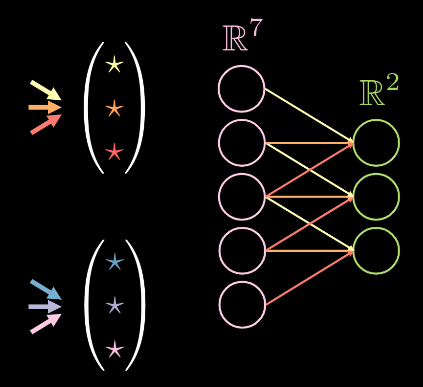
\includegraphics[width=200pt]{labs/03/images/kernel.png}
            \end{center}
            \captionsetup{justification=centering, margin=2cm}
            \caption{Example of parameter sharing using kernels. Colored connections refer to kernel space}
            \end{figure}
            
    \end{enumerate}
    
    \section{Resulting Improvements}    
    % Authors: Rafael Moraes, Jiachen Zhu, Kabir Singh; 2019-02-19
    The use of Sparsity and Parameter Sharing leads to:
    \begin{enumerate}
        \item \textbf{Faster convergence} \(\rightarrow\) Fewer weights to tune and ability to optimize the same parameters using multiple parts of the network/data.
        \item \textbf{Better model generalization}\(\rightarrow\) Fewer parameters leads to less overfitting.
        \item \textbf{Models not constrained to input size}\(\rightarrow\)Can keep applying same sets of parameters to small regions of the input independent to its size.
        \item \textbf{Kernel independence}\(\rightarrow\) leads to higher parallelization capabilities.
        \item \textbf{Reduced amount of computation}\(\rightarrow\) efficiency! 
    \end{enumerate}
    
    \section{Notes}
    % Authors: Rafael Moraes, Jiachen Zhu, Kabir Singh; 2019-02-19
    Two important aspects to keep in mind:
    \begin{itemize}
        \item \textbf{Kernel Format}: In PyTorch, the order that the kernels are stored in the tensor is:
        \begin{equation}
            \underset{\# kernels}{\mathrm{N}} \times
            \underset{\# channels}{\mathrm{C}} \times
            \underset{h \times w \text{ of kernel}}{K}
        \end{equation}

        \item \textbf{Zero-Padding}: Operation of introducing zeros to the borders of the input.
        It is commonly used in order to maintain the size of the input in the output after a convolutional transformation.
    \end{itemize}
    
